% !TEX root = /home/qtbodart/Git/Work/UCLouvain/FYKI/LMAPR1230/Synthèses/Synthese.tex
\documentclass{article}
\usepackage{graphicx} % Required for inserting images
\graphicspath{ {./Images/} }
\usepackage{amsmath}
\renewcommand{\familydefault}{\sfdefault}

\title{Synthèse LMAPR1491}
\author{Quentin Bodart}
\date{Q1 2024-2025}

\begin{document}
\maketitle
\tableofcontents
\pagebreak

\section*{Compétences visées}
    \begin{itemize}
        \item Utiliser correctement le langage de la chimie et plus
        particulièrement celui de la chimie organique.
        \item Comprendre les relations entre la nature, la
        structure et les propriétés de composés organiques.
        \item Prédire et analyser la réactivité de composés
        organiques donnés.
        \item Pouvoir utiliser les notions théoriques apprises au
        cours pour résoudre des exercices.
    \end{itemize}

\section{Introduction et rappels}
    \subsection{La chimie organique}
        La chimie organique est une branche de la chimie qui concerne
        l’étude et la transformation de molécules d’origine pétrolière ou
        vivante contenant principalement
        du carbone, de l’hydrogène, de l’oxygène et de l’azote.\\\\
        Elle prend ses débuts dans la création accidentelle d'urée par Friedrich Wöhler en 1828.
        Cette découverte mit fin à la théorie "vitaliste" (seule la nature est capable de synthétiser des molécules organiques) 
        et marque le début de la synthèse artificielle de ces molécules.

    \subsection{Le carbone}
        \subsubsection{Pourquoi le carbone?}
            Pourquoi le carbone est-il prépondérant dans la chimie organique ? \\
            D'autant plus que carbone est très peu abondant à l'échelle de l'univers (0,06 \%) !

            \begin{itemize}
                \item La liaison C-C est particulièrement forte (+- 350 kJ/mol, contre 230 pour Si-Si, 146 pour O-O, ...)
                \item Les liaison C=C sont moins fortes que C-C, ce qui fait que le carbone tend 
                    à former de longues chaînes (contrairement aux autres atomes)
                \item Il se lie très fort avec H
            \end{itemize}
            Donc, l'état "préféré" du carbone est une longue chaîne, parfois branchée 
            et se repliant sur elle-même, et fortement liée avec des atomes d'hydrogène.
        
        \subsubsection{Hybridation}
            Les liaison du carbone ne peuvent pas simplement 
            s'expliquer via ses électrons de valence !
            Le carbone s'hybride, formant des orbitales $sp$, $sp^2$ ou $sp^3$ ! \\
            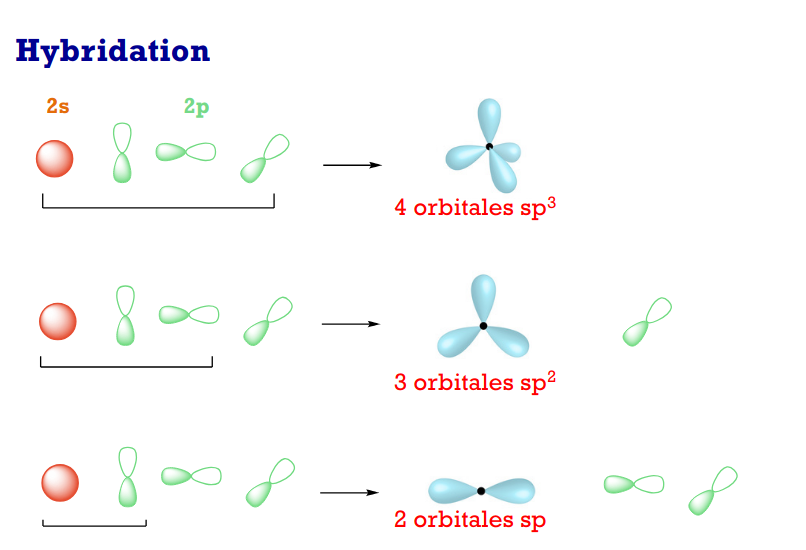
\includegraphics[scale=.5]{hybridation_carbone.png} \\
            Les orbitales $p$ restantes vont former des liaisons 
            nommées $\pi$ entre elles, tandis que les orbitales $sp$ 
            vont se lier en formant de liaisons $\sigma$. \\\\
            La liaison C=C généralement formée d'une liaison $\pi$ 
            et d'une liaison $\sigma$ :\\
            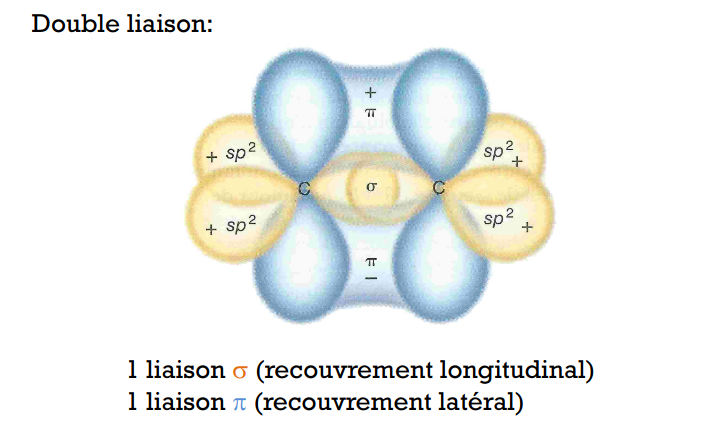
\includegraphics[scale=.5]{liaison_double_c_c.png}\\\\
            La liaison C$\equiv$C, quant à elle, est généralement 
            formée de deux liaison $\pi$ et d'une liaison $\sigma$ : \\
            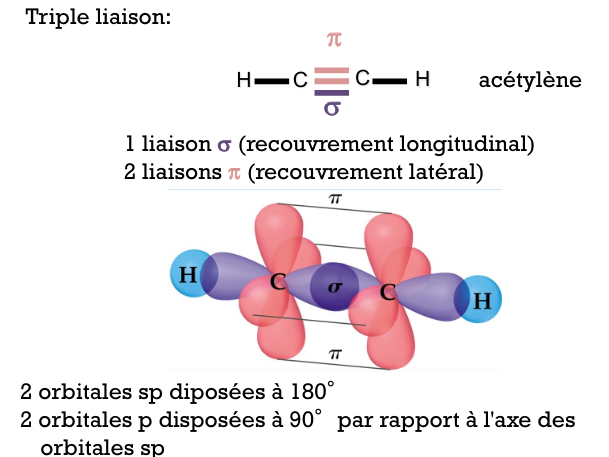
\includegraphics[scale=.5]{liaison_triple_c_c.png}

        

    \subsection{Théorie VSEPR}
        La \textbf{théorie VSEPR} (\textbf{V}alence \textbf{S}hell \textbf{E}lectron \textbf{P}air \textbf{R}epulsion)
        vise à prédire la géométrie d'une molécule en se basant sur les
        répulsions entre paires d'électrons. \\\\
        On y considère qu'un atome est entouré d'électrons de valences répartis 
        par \textbf{paires}, et que la molécule tente d'adopter une 
        géométrie \textbf{minimisant la répulsion entre ces paires} :\\
        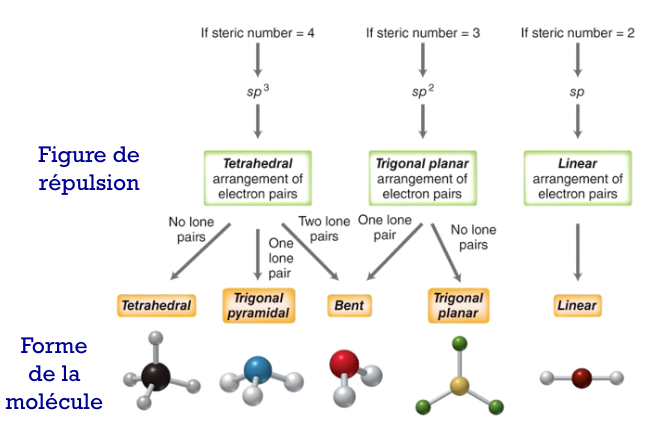
\includegraphics[scale=.7]{VSEPR.png}

    \subsection{Représenter une molécule}
        \subsubsection{Formules}
            Il y a plusieurs manières de représenter une molécule :
            \begin{itemize}
                \item Formule Brute : Liste simplement les atomes présents \\
                Exemple : $C_2 H_6 O$, $C_3 H_6 Cl_2$, ... 
                \item Formule Semi-dévellopée : Liste les atomes dans l'ordre de la chaîne principale \\
                Exemple : $CH_3CH_2OH$, $CH_2ClCHClCH_3$, $CH_3CH_2CH_2CH_2CH_3$, ... 
                \item Formule dévellopée plane (structure de Lewis) : Représente les molécules à plat et les liaisons entre groupements (Expliquée plus bas)\\
                Exemple :\\
                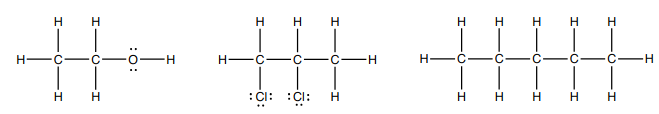
\includegraphics[scale=.6]{structures_planes.png}
                \item Formule simplifiée (ou topologique) : chaque coin représente un carbone lié à un maximum d'atomes d'hydrogène \\
                Exemple :\\
                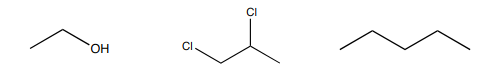
\includegraphics[scale=.8]{formule_topologique.png}
            \end{itemize}
        
        \subsubsection{Structure de Lewis}
            Elle se base sur la règle de l'octet, et permet de représenter les \textbf{charges formelles} : \\
            % TODO
            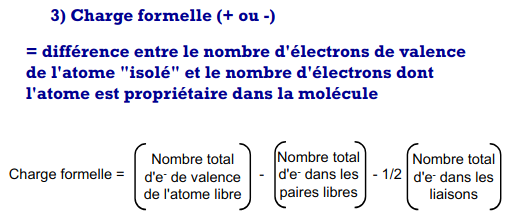
\includegraphics{charge_formelle.png}

    \subsection{Les hydrocarbures}
        \subsubsection{Les alcanes}
            Les alcanes sont des chaînes de C simplement liés et saturés en atomes d'hydrogène. \\
            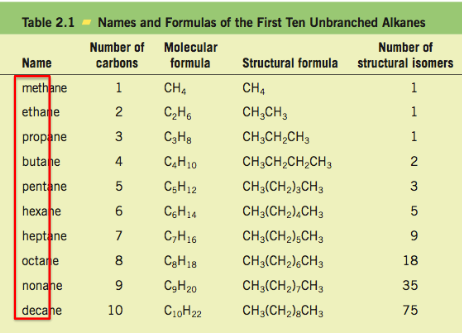
\includegraphics{nomenclature_alcanes.png}
        
        \subsubsection{Nomenclature}
            La nomenclature des alcanes passe par les
            règles \textbf{IUPAC} (International Union for Pure and Applied Chemistry) :\\
            \begin{itemize}
                \item Le préfixe est lié à la longueur de chaîne.
                \item Le suffixe “ane” signifie hydrocarbure saturé.
                \item On sélectionne la chaîne la plus longue.
                \item On numérote cette chaîne de façon à avoir les plus petits chiffres
                possibles pour spécifier la position des substituants
                \item Les substituants sont affectés du numéro(s) du (des) carbone(s)
                porteur(s) pour les localiser
                \item Les préfixes di-, tri-, tétra-,… sont utilisés si un même substituant
                est présent plusieurs fois
            \end{itemize}

        \subsubsection{Groupes alkyles}
            Les ramifications à base de C et H retrouvés autour de la chaîne principale sont des \textbf{groupes alkyles} :\\
            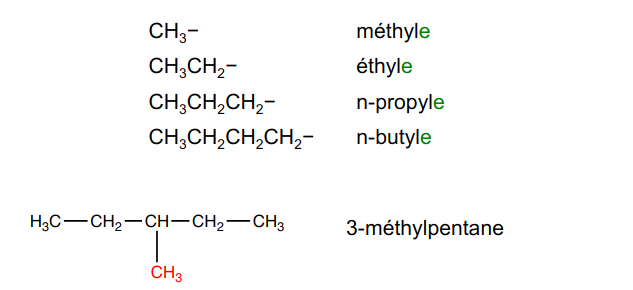
\includegraphics[scale=.4]{groupes_alkyles.png}
            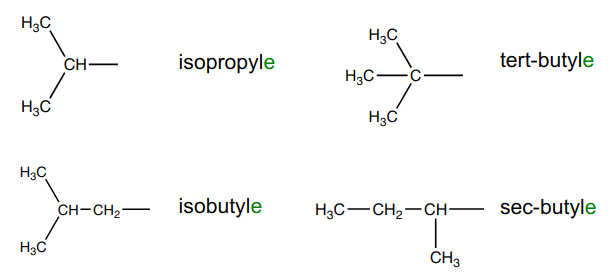
\includegraphics[scale=.4]{groupes_alkyles_particuliers.png}

        \subsubsection{Alcanes Cycliques}
            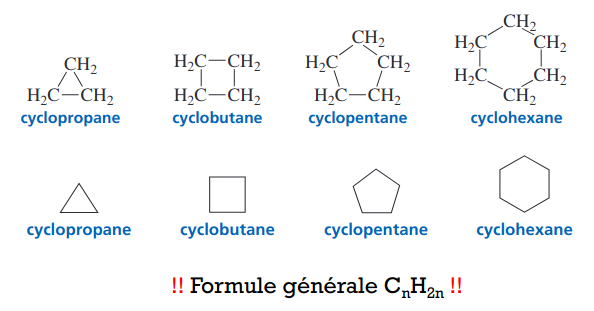
\includegraphics{alcanes_cycliques.png}
        
        %TODO
    \pagebreak
    \subsection{Les groupes fonctionnels}
        \begin{itemize}
            \item Alcools : $R-OH$, Si R = C $sp^2$, on parle d'\textbf{énol}.
            \item Ethers : $R-O-R'$
            \item Amines : $N-R_3$
            \item Cétones : \\ 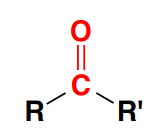
\includegraphics[scale=.5]{cetone.png}
            \item Aldéhydes : \\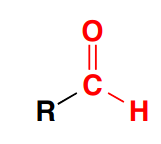
\includegraphics[scale=.5]{aldehyde.png}
            \item Acides carboxyliques : \\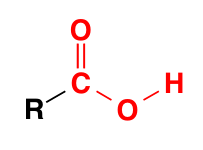
\includegraphics[scale=.5]{acide_carboxylique.png}
            \item Esters : \\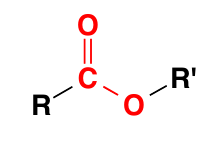
\includegraphics[scale=.5]{ester.png}
            \item Amides : \\
            %TODO
        \end{itemize}
\end{document}